\section{Literature review}\label{sec:review}
In this chapter, previous work on the optimisation of network tied-arch bridges related to the introduced problem is summarized. However, the field is rather young in general, and further, most emphasis has been placed on the hanger arrangement pattern over the density. Nevertheless, the studies on the hanger arrangement pattern are of relevance to this Thesis, as the density is linked to the arrangement and the same methods are suitable for either investigation. In most studies, a single aspect is investigated, such as hanger unloading or the hanger forces in general, fatigue or cable loss. These aspects, which are investigated in parametric studies, are introduced in Sections \ref{sec:rev_forces} to \ref{sec:rev_loss}. Besides parametric studies, numerical optimisation methods have been used not just to identify the tendencies, but to further optimise the choice of parameters in the continuous domain. Recently, these methods have been used to minimise the weight or even the costs of a network tied-arch structure. The respective studies are introduced in Sections \ref{sec:rev_weight} and [!!!]. Few authors have taken a further step and introduced a design methodology allowing for a fast and approximately optimized initial design. These methods, which are evaluated critically, are presented in Section \ref{sec:rev_meth}. Ultimately, the Master Thesis of Riccardo Cavegn, which builds the foundation of this Thesis, is summarized in Section \ref{sec:rev_prev} and a summary of this chapter is given in Section \ref{sec:rev_sum}.

\subsection{Hanger forces} \label{sec:rev_forces}
Per Tveit, described the concept of network tied-arch bridges in his dissertation in 1959 and designed two of the first bridges of this type in 1963 in Norway.
%[History] Since then, he has been giving lectures around the world to contribute to the broader use of network tied-arch bridges. He points out the various advantages over vertical hangers in terms of lower steel weights, simple detailing and the good use of strong materials \citep{Tveit}. He recommends constant hanger spacing on the arch with one hanger per node to minimize the bending moments in the arch. 
He also conducted investigations on the hanger arrangement, aiming to prevent hanger unloading which is a critical issue under asymmetric loading for short-span bridges \cite{Tveit3}.
In these early stages, only the parallel hanger net and the constant change of inclination pattern were used. 
It was found that whereas flat inclinations are more suitable to prevent hanger unloading, they also result in higher hanger forces. To find a solution for these opposing objectives he developed diagrams, which predict the maximum hanger inclination without hanger unloading depending on the ratio of life to dead loads. As a first optimisation of the hanger arrangement, he proposed to increase the inclinations of the hangers as much as possible before the first hanger unloading occurs. \medskip

In 2012, Teich conducted a vast parameter study varying the key in-plane parameters to investigate the hanger force-related objectives \cite{Teich}. Namely, these objectives are the maximum force, its variation, the cyclic stresses and the amount of unloaded cables, without considering the three hangers closest to the knuckle. The parameters such as the span, the rise, the amount of hangers and their arrangement are varied in the study, leading to a total of approximately \SI{90000}{} variants. The only in-plane parameter which is left constant is the circular arch shape. The cross-sections of the arch rib and the tie girder were obtained in a simplified preliminary design assuming a steel carriageway. Each variant was then analysed in a two-dimensional model under unilateral and full vertical train live loading. 
Again, hanger unloading posed a big issue for many variants and affected all investigated objectives. Therefore, Teich recommends the arrangement of 36 to 52 hangers per plane for spans between \SI{100}{m} and \SI{250}{m}. Further, he recommends flat inclinations between $50\degree$ and $55\degree$ for the parallel hanger pattern. The constant change of inclination arrangement offers significant advantages and relies on large changes of inclination. However, the radial arrangement with an intersection angle $\beta=36\degree$ was found the best regarding virtually all the considered objectives. Based on the normalized and combined objectives, Teich also developed a design methodology, which is explained in Section \ref{sec:rev_meth}. \medskip

It has to be noted, that both Tveit and Teich did not consider prestressing of the hangers in their models. It is implicitly assumed, that the permanent hanger forces correspond to the elastic response under permanent loads. Also, the ratio of live to dead loads is assumed to be particularly high (up to $p/g=1$). Therefore, the impact of hanger unloading is significantly overestimated compared to common network tied-arch bridges featuring a concrete deck.
%results normalized and mixed multiple times.

\subsection{Fatigue} \label{sec:rev_fat}
Pellegrino et al. evaluated hanger patterns with respect to fatigue on a bridge featuring a composite deck and a life to dead load ratio of $p/g=0.3$ and a span of \SI{100}{m} \cite{Pellegrino}. The considered hanger patterns are the constant change of inclination and the radial arrangement which are also compared to a vertical arrangement. It is found that with respect to the maximum and the average cyclic stresses, vertical hangers are advantageous over network arrangements. By inclining the vertical hangers the behaviour deteriorates strongly and improves again for flat inclinations. Especially the flat hangers of the radial arrangement near the knuckle undergo very high cyclic stresses and various modifications to reduce the maximum cyclic stress are studied. However, no generally applicable modification independent of the intersection angle was found. Therefore, it is recommended to design the hangers near the knuckle independent of the hanger arrangement pattern. Steeper hangers near the knuckles are generally a good advice to start with. For a radial hanger arrangement with 22 hangers per set, it is recommended to arrange the last five hangers of each set parallel to the previous one, as shown in \autoref{fig:Pellegrino}.
\begin{figure}[H]
    \centering
    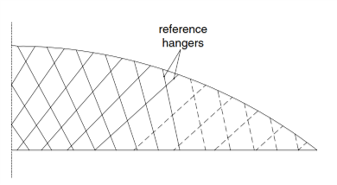
\includegraphics[width=0.5\textwidth]{Pictures/PellegrinoArrangement.png}
    \caption{Modified radial arrangement \cite{Pellegrino}}
    \label{fig:Pellegrino}
\end{figure}


\subsection{Cable loss} \label{sec:rev_loss}

Most of the work dedicated to cable loss focuses on cable-stayed bridges, for which it is not unusual, that the design of the superstructure is governed by this accidental limit state. Wolff and Starossek found, that the loss of two or more cables can even impair the global stability of a cable-stayed bridge \cite{Wolff}. In an investigation on the Blennerhassett Island Bridge, Zoli and Woodward showed that a network tied-arch bridge offers more redundancy and can even withstand the loss of multiple cables \cite{Zoli}. However, it is concluded that cable loss should be a key consideration for the design process for all major network tied-arch bridges. Further they point out that a detailed dynamic analysis can allow for a significant reduction of the dynamic amplification factor due to cable loss.\bigskip

Bruno et al. conducted a study on the behaviour of network tied-arch bridges to identify the key factors on the effects under cable loss \cite{Bruno}. The behaviour is studied using the simplified approaches of the PTI and the Eurocode and compared to a dynamic non-linear FE-analysis \cite{PTI}. As a reference case, a bridge with a span of \SI{180}{m} and a rise of \SI{30}{m} is studied featuring a parallel hanger arrangement with 17 hangers per set and an inclination of $65 \degree$. Further, prestressing is taken into account using the zero-displacement method. It was found that the most dangerous cables to lose are the ones located near the quarter points of the tie and are inclined towards the crown of the arch. The corresponding vertical displacements are maximal for this hanger with a value of $l/4000$. The stresses in the neighbouring hangers of the same set increase by 60\%, if the cable at the quarter point is lost. The hangers of the other set are less affected increasing by a maximum of less than 25\% as shown in Fig. \ref{fig:Bruno}. It is concluded, that also the simplified method by the PTI provide an adequate degree of accuracy, as they only underestimate the hanger forces in the less affected hanger set.
\begin{figure}[H]
    \centering
    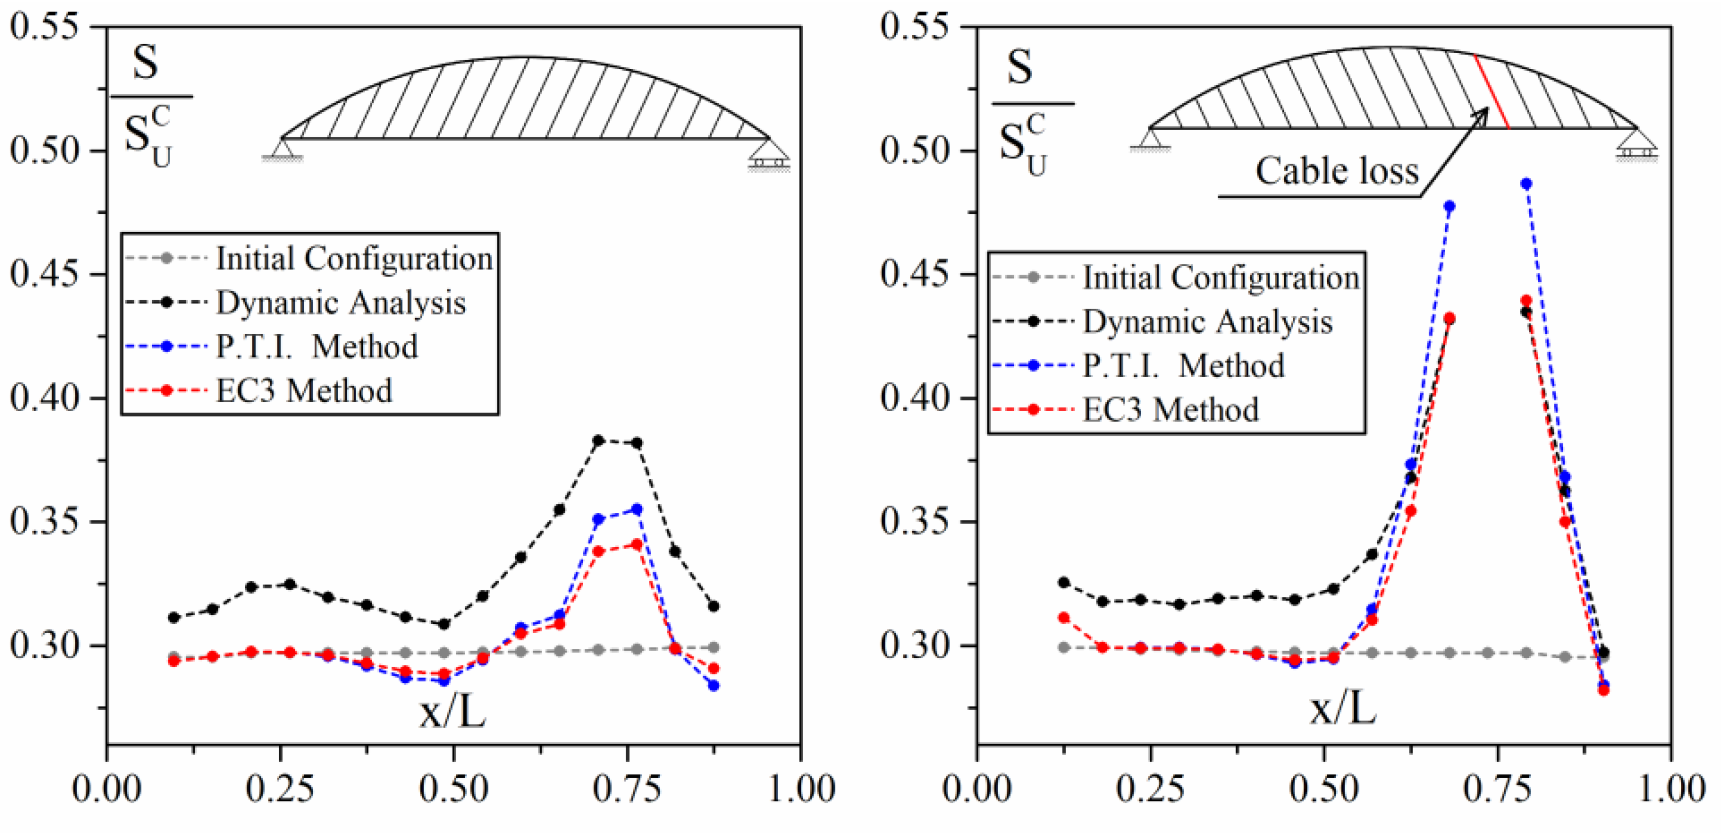
\includegraphics[width=0.75\textwidth]{Pictures/BrunoCableLoss.PNG}
    \caption{Stress distribution in the hanger sets \citep{Bruno}}
    \label{fig:Bruno}
\end{figure}

Further, it was found that parallel arrangements with flatter inclinations cause the displacements and the internal forces to increase. Restricted to the plausible range of $50\degree$ to $70\degree$, differences in the deflections amounting up to 20\% can be expected. In Fig. \ref{fig:Bruno2} the respective displacements are also compared to the arrangement with vertical hangers, where also the resulting total volumes of the hangers are given. It is seen that the vertical arrangement performs significantly better despite using a smaller quantity of cable material. Compared to the investigations on hanger forces and fatigue, an opposite tendency is observed, where the behaviour improves for steeper hangers. This is due to the stiffer behaviour of steep hangers.
\begin{figure}[H]
    \centering
    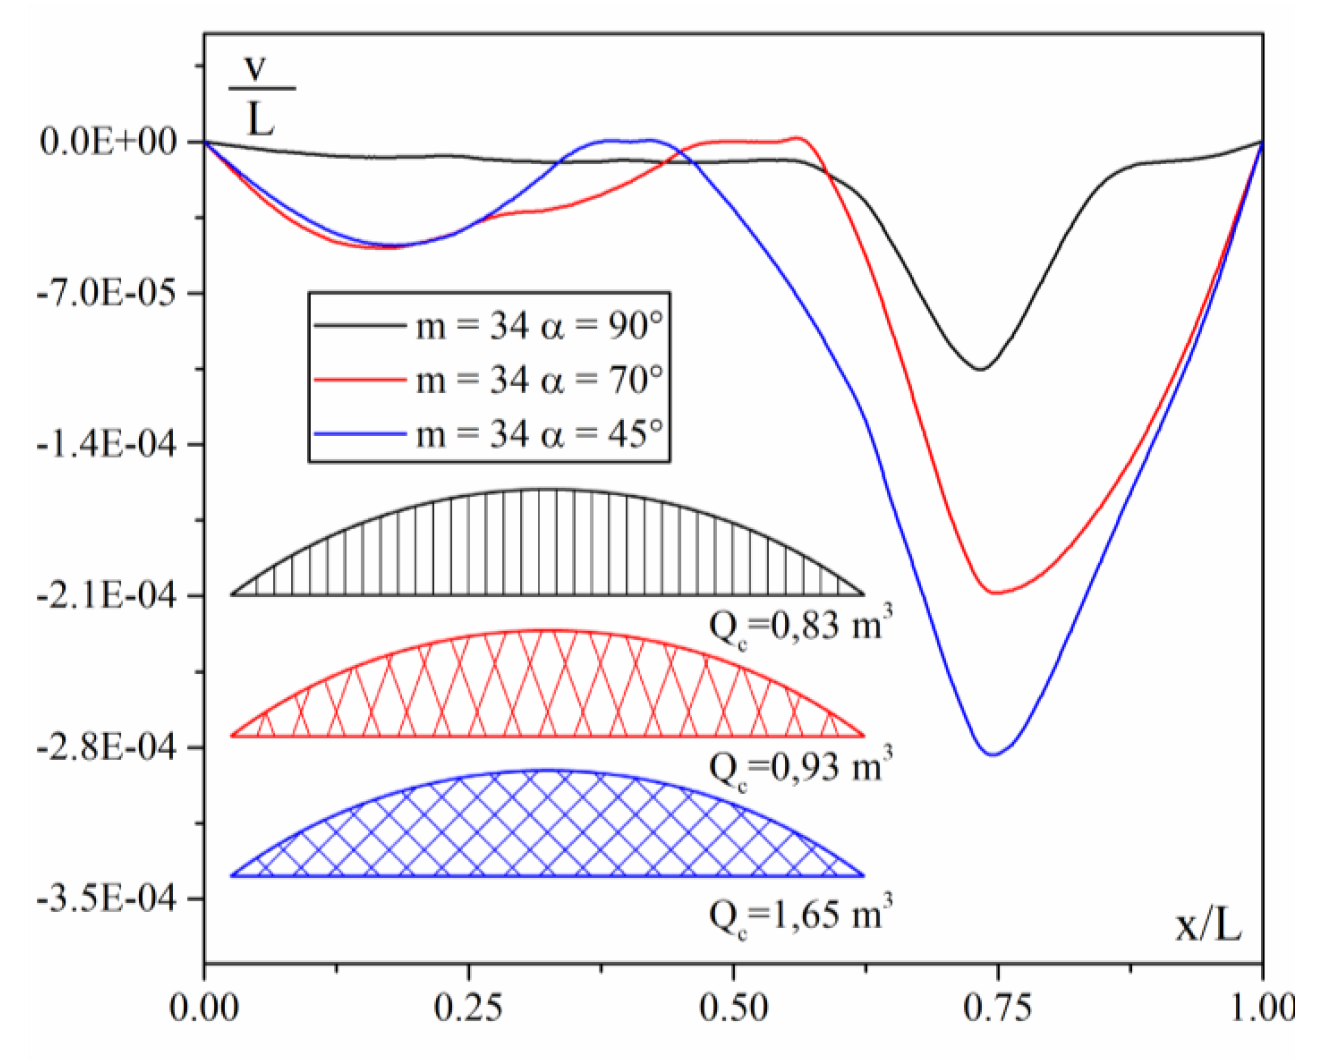
\includegraphics[width=0.6\textwidth]{Pictures/BrunoArrangements.PNG}
    \caption{Vertical deflections under cable loss \citep{Bruno}}
    \label{fig:Bruno2}
\end{figure}

\subsection{Structural weight} \label{sec:rev_weight}
Recently, many researchers have focused on numerical optimisation methods over parametric studies. Technically, all parameters describing the scheme of a network tied-arch bridge can be considered. However, as it is usually not the aim to optimise a full design, researchers prefer to limit the process to a few key variables. As some of the parameters are of discrete form, the problem is mathematically described as a constrained mixed-integer problem. Genetic algorithms with penalisation provide an efficient and often used tool for these problems. Belevicius et al. optimised a pedestrian bridge with respect to the weight for different boundary conditions \cite{Belevicius}. Even with the rather limited amount of nine parameters, the optimized sets are well dispersed over the feasible domain, accentuating the multi-modality of the underlying problem.
It also demonstrates the difficulties associated with numerical optimisation for design purposes. Even after reducing the amount of parameters, the results do not resemble typical tied-arch bridges, be it for the high amount of hangers or the large rise-to-span ratios. Ultimately, a strongly varying hanger pattern is recommended as well as a rise-to-span ratio of up to 0.23. The aim of finding a simple and fast method for obtaining the full initial design is therefore reached only in an unsatisfactory manner.
It is likely, that an oversimplified objective function yielded these odd designs, as the unfactored weights neglect the differences in the unit costs, which favours the arrangement of additional hangers in particular.

\subsection{Structural costs}
Design optimisations often take the goal of minimising the structural costs as an objective. Recently, researchers have used a wide range of optimisation methods to solve problems with geometrical, topological and mechanical design variables underlying different sets of structural constraints \cite{MARTINS}. However, the main focus of the field lies again on cable-stayed bridges, and further, only a single publication attempted to take the construction expenses into the objective. It is key to remember, that for the slender network tied-arch bridges a high ratio of the costs is made up by labor and not by the material and the fabrication of the components \cite{Tveit2}. Therefore, the estimated structural costs can serve well as a guideline, however it makes sense, to keep the focus on the structural considerations.

\subsection{Design methodologies} \label{sec:rev_meth}
The complex behaviour of the network tied-arch bridge is at least partially responsible for its comparably sparse use \cite{Tveit2}. As an engineer does not have the capacity to run a full optimisation, design guidelines or methodologies are key to promote the construction of this bridge type. However, only few authors have attempted to tackle this challenge for network tied-arch bridges.

Teich developed a design methodology based on the results of a vast parameter study. In a first step, the number of hangers is chosen according to the recommended values depending on the span of the bridge, shown in [Figure]. Using the amount of hangers and the span, the optimal hanger arrangement pattern is chosen using a different table, in which the arrangements are ranked according to their normalised score. For all cases either the constant change of inclination or the radial arrangement are the preferred choice. Ultimately, the best set of parameters can be chosen depending on the amount of hangers in a table corresponding to the respective hanger set. An example for the radial arrangement is shown in [Figure]. The three hangers closest to the knuckle should ultimately be designed manually. 

Whereas this methodology is fairly simple to use, it lacks a specific boundary of application. For the span of the Blennerhassett Island Bridge, a minimum amount of 42 hangers is recommended, which is almost twice as many as were actually designed. This overestimation is partially due to the live to dead load ratio close to $p/g=1$ in the analysis underlying the methodology. Further, only normal forces were considered to judge the optimality of the structure. This is a great oversimplification of the actual objective of an optimised design.\medskip

To overcome the numerical challenges of the generally often used metaheuristic optimisation methods, Bruno developed a three-step analysis \cite{Bruno}. Starting with an initial design, the zero-configuration is determined by a method similar to the zero-displacement method, yielding the individual prestressing forces and hanger areas. In a second step, the structure is analysed under the action of live loads. If the design conditions are not verified, the stiffnesses of the hangers, which are treated individually, are adapted. Next, the arch rib and the tie girder can be designed on the obtained distributions of internal forces. This procedure is repeated until the changes lie within a certain tolerance.[Wieso auch diese methode unbrauchbar ist...]

\subsection{Previous work in this series} \label{sec:rev_prev}
In a previous Master's Thesis at the Chair of Structural Engineering for Concrete Structures and Bridge Design, Riccardo Cavegn investigated the optimal arch geometry \cite{Cavegn}. Its dependency on the hanger arrangement was studied in particular, with the Blennerhassett Island Bridge as a reference bridge. The constant change of inclination arrangement as well as its subset, the parallel arrangement, were optimised and analysed in a parameter study. 
In the first step, the prestressing of the hangers was determined to minimize the bending moments under dead loads. To achieve this, the hanger tuning matrix relating the individual unit strains of the hangers to the bending moments along the tie girder was calculated using structural analysis software. This matrix was then used to determine the prestrains giving minimal bending moments as shown in \autoref{fig:Cavegn3}. In a second step, the obtained hanger forces forces were used to graphically construct the thrust line of the arch as illustrated in \autoref{fig:Cavegn4}. As the two steps influence each other, they are repeated until the obtained arch geometry stabilises.
\begin{figure}[H]
\centering
\begin{subfigure}{0.5\textwidth}
    \centering
    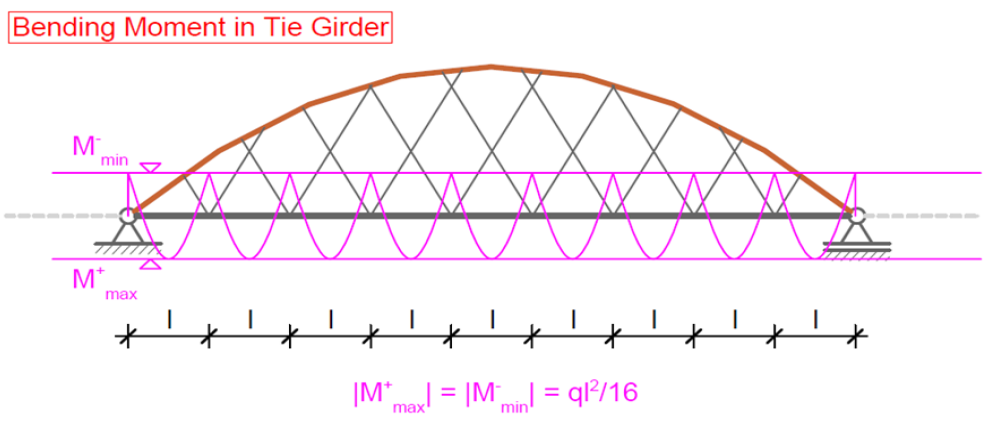
\includegraphics[width=0.73\textwidth]{Pictures/OptimizedBendingMoment.PNG}
    \caption{Determination of the self-equilibrium stress state}
    \label{fig:Cavegn3}
\end{subfigure}%
\begin{subfigure}{.5\textwidth}
    \centering
    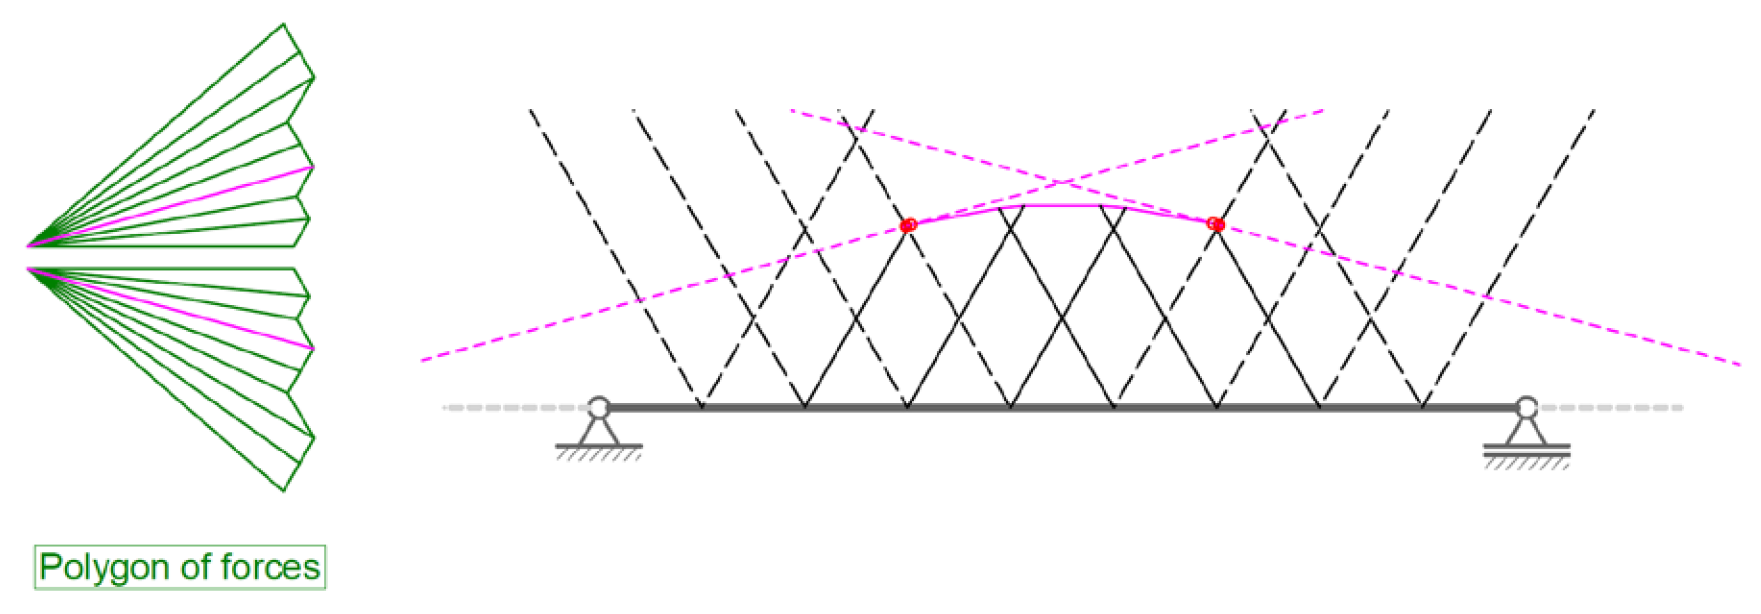
\includegraphics[width=0.9\textwidth]{Pictures/GraphicalThrustLineConstruction.PNG}
    \caption{Graphical construction of the arch shape}
    \label{fig:Cavegn4}
\end{subfigure}
\caption{Optimisation steps \cite{Cavegn}}
\label{fig:Cavegn34}
\end{figure}
It was found, that the obtained arch geometries generally do not correspond to the circular or the parabolic shape. Sometimes they even lie outside of the two traditionally used shapes. By approximating the obtained shape with a quartic function, an analytical expression close to the thrust line was found, deviating by a maximum of 2\% of its height for most arrangements. Further, it was seen that flat angles of inclination lead to thrust lines that are more inclined near the bearing. Ultimately, the impacts under the unilateral live load combinations were used to estimate the costs of the generated structure in a comparative study. The final design of the Blennerhassett Island Bridge was taken as a reference and its cost was estimated using unit prices and the quantities specified in the design drawings. The cost of each component in the investigated designs was estimated proportionally to the respective elastic stresses. A flatter hanger inclination turned out to reduce the bending moment in the tie and the arch, whereas the maximum hanger forces increased. The estimated costs of the bridge were reduced the most by decreases of inclinations and high initial inclinations. The cost function is thereby minimised by up to 12\%. However also other patterns, e.g. with constant inclination, performed well if the arch geometry is adapted to the thrust line.


\subsection{Summary} \label{sec:rev_sum}
Along with the increase in popularity of network tied-arch bridges, researchers have investigated its manifold aspects. Starting from the hanger forces, which were aimed to be uniform and safe from unloading, the behaviour under fatigue loading and cable loss has been studied. As each of these aspects necessitates a detailed consideration, not one integral design optimisation has been conducted for a network tied-arch bridge. On top of that, the findings of these investigations favour divergent design parameters and there are varying boundary conditions, such as the live to dead load ratio, which complicate the formulation of general guidelines. In this challenging environment, it is tempting to combine the objectives into a single score, be it from the results of a parametric study or as an objective function for an optimisation method. However, both Teich and Belevicius have exemplified, that this approach does not solve the challenges, it only obfuscates the impact of the design variables on the structural behaviour. The lack of knowledge about this bridge type is still too big for the use of advanced optimisation methods to yield a suitable design. While focusing on the costs of the structural components helps putting different aspects into perspective, it should be remembered that the cost of labour outweigh material and fabrication costs. Ultimately, Cavegn pointed out, that key design considerations, such as the self-equilibrium stress state and the arch shape, have only been addressed in an unsatisfying manner. 


%Further it was pointed out early by \citep{Geissler} that only with a detailed structural model, including accurately modelled knuckles, reliable estimations of the hanger forces can be made.






%\subsection{Hanger arrangements}
%\paragraph*{Hanger unloading}
%Later, he proposed an arrangement with constant distances between the hanger connection points in the middle of the tie, as shown in \autoref{fig:Tveit}. While the nodes on the arch are spaced equidistantly, the connection points on the tie are constructed with the help of an inclined ellipse and an abscissa and an ordinate depending on the parameters $p_1$ and $p_2$. To determine the points on the tie, linearly spaced vertical lines are drawn to the ellipse. The locations of the nodes on the tie are then determined from the ordinate values of the intersection points.\\
%\begin{figure}[H]
%\centering
%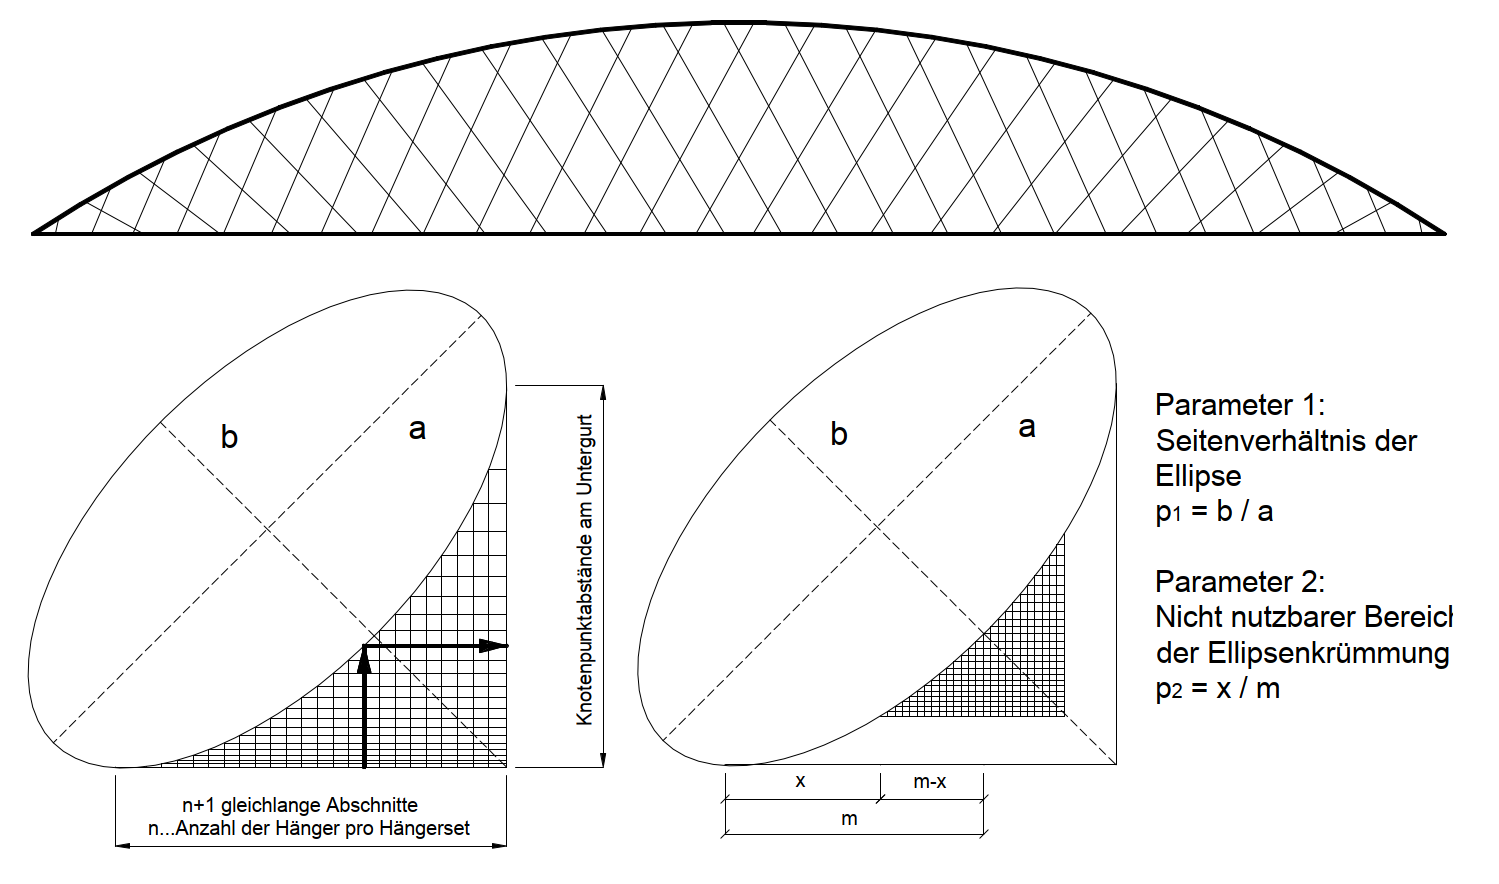
\includegraphics[width=0.7\textwidth]{Pictures/ArrangementTveit.PNG}
%\caption{Arrangement with constant distances in the middle of the tie (adopted from \cite{Teich}).}
%\label{fig:Tveit}
%\end{figure}

%In \citep{Tan} a pedestrian bridge with a sparse hanger arrangement was investigated using an evolutionary optimisation procedure. Each hanger is arranged independently of an overall arrangement. It was found that an arrangement approximately consisting of two separate patterns reduced the internal forces in the arch and the tie the most. Near the knuckles vertical hangers and in the span approximately parallel hangers resulted as shown in \autoref{fig:Tan}.
%\begin{figure}[H]
%\centering
%\begin{subfigure}{0.5\textwidth}
%    \centering
%    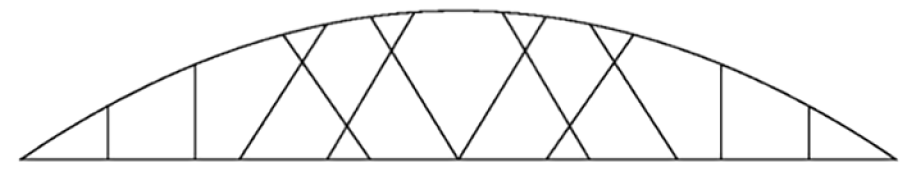
\includegraphics[width=0.9\textwidth]{Pictures/Tan 1.PNG}
%\end{subfigure}%
%\begin{subfigure}{.5\textwidth}
%    \centering
%    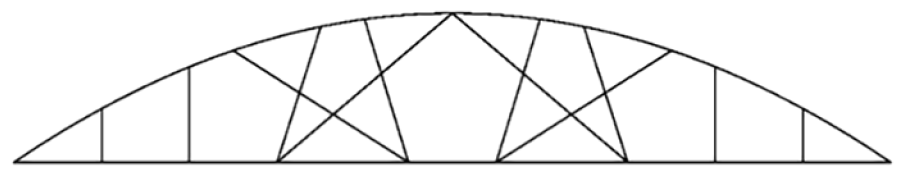
\includegraphics[width=0.9\textwidth]{Pictures/Tan 2.PNG}
%\end{subfigure}
%\caption{Optimal sparse hanger arrangements (adopted from %\cite{Tan}).}
%\label{fig:Tan}
%\end{figure}

\paragraph*{I don't know}
In the new millennium, Tveit supervised multiple Master Theses aiming to optimize the design of network tied-arch bridges. In \citep{BrunnSchanack} [nochmals lesen was da genau gemacht wurde]. They developed the radial arrangement aiming to have a pattern which optimally complies with a circular arch. In the radial arrangement, the hangers are equally spaced on the arch and two following hangers cross each other symmetrically to the radius as shown in \autoref{fig:Brunn}. It was the intention, that if the hanger forces are uniform, the thrust line also approximately corresponds to a circle, resulting in an efficient use of the arch. In the literature, this arrangement is either described by the angle $\alpha$ between the arch and the hanger or by the angle $\beta$ between the hangers and the radius at the first intersection point.

\begin{figure}[H]
\centering
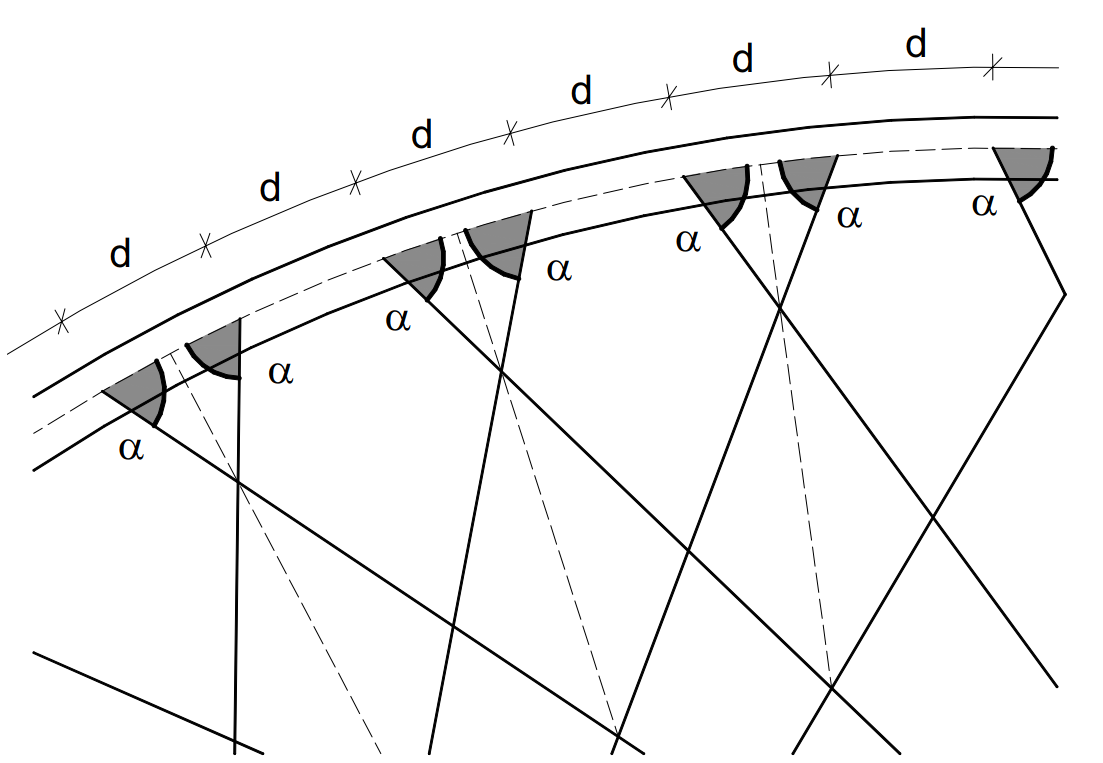
\includegraphics[width=0.4\textwidth]{Pictures/RadialArrangement.PNG}
\caption{Radial hanger arrangement (adopted from \citep{BrunnSchanack2}).}
\label{fig:Brunn}
\end{figure}

Both of the authors continued their work in the field of network tied-arch bridges and conclude their findings in \citep{BrunnSchanack2}. Besides the bending moments and the maximum hanger forces, also the variation of hanger forces, which are relevant for fatigue, and the elastic embedding of the arch is focused on. These objectives are evaluated manually/arbitrarily. In a comparison of the different hanger patterns, it is concluded that parallel hangers are disadvantageous concerning the bending moments in the arch as the hanger forces vary strongly. Angles of inclination between $55\degree$ and $60\degree$ give the best results. For the constant change of inclination arrangement the middle hanger was recommended to be inclined in the similar range from $56\degree$ to $60\degree$. Further, the change of inclination between two following hangers should lead to an inclination of up to $80\degree$ in the steepest hangers. The radial arrangement was considered optimal, especially for the small corresponding variation of maximum hanger forces and uniform embedding of the arch. The angle between the hangers and the arch are recommended to be between $55\degree$ and $60\degree$. Interestingly, the optimal solutions for each hanger arrangement feature a middle hanger with an inclination of $55\degree$ to $60\degree$. Further, it is recommended that the hanger spacing on the arch lies between \SI{2.5}{m} and \SI{4}{m}.

